%%%%%%%%%%%%%%%%%%%% author.tex %%%%%%%%%%%%%%%%%%%%%%%%%%%%%%%%%%%
%
% sample root file for your "contribution" to a proceedings volume
%
% Use this file as a template for your own input.
%
%%%%%%%%%%%%%%%% Springer %%%%%%%%%%%%%%%%%%%%%%%%%%%%%%%%%%


\documentclass{svproc}
%
% RECOMMENDED %%%%%%%%%%%%%%%%%%%%%%%%%%%%%%%%%%%%%%%%%%%%%%%%%%%
%

% to typeset URLs, URIs, and DOIs
\usepackage{url}
\usepackage{float}
\usepackage{graphicx}
\usepackage[section]{placeins}
\usepackage{amsmath}
\usepackage{amssymb}
\def\UrlFont{\rmfamily}

\begin{document}
\mainmatter              % start of a contribution
%
\title{Multiobjective Node Immunisation of Complex Networks}
%
\titlerunning{Multi-Objective Node Immunisation}  % abbreviated title (for running head)
%                                     also used for the TOC unless
%                                     \toctitle is used
%
\author{Joost Nibbeling}
%
\authorrunning{Joost Nibbeling et al.} % abbreviated author list (for running head)
%
%%%% list of authors for the TOC (use if author list has to be modified)
\tocauthor{Joost Nibbeling}
%
\institute{Leiden Institute of Advanced Computer Science, Leiden University, Netherlands}

\maketitle              % typeset the title of the contribution

\begin{abstract}
Node immunisation is selecting nodes for removal from a network or graph to make it more robust against virus attacks. It is a problem of high societal relevance, for example in epidemiology. We measure the effect on immunisation by the drop in the maximum eigenvalue or eigen-drop. The $k$-node immunisation problem  has been proven to be NP-hard. Several heuristics have been developed to approximate the problem. In this work we  focus on a multiobjective variant of the problem that can take into account immunisation cost instead of requiring a value of $k$ to be known a priori. To approximate the Pareto fronts of the problem, we introduce extensions to  the NetShield and NetShield+ algorithms. In addition we also approximate the Pareto fronts with two genetic algorithms. For this we use two graphs from literature and two graphs sampled from graph models. Insight into the shape of the Pareto fronts and under which circumstances which methods work best is gained, which can help find quicker and better solutions to immunisation of real work networks, such as occur in epidemiology.

% We would like to encourage you to list your keywords within
% the abstract section using the \keywords{...} command.
\keywords{Immunisation, Multiobjective Optimisation, ShieldValue, Genetic Algorithms}
\end{abstract}
%
\section{Introduction}
%

The immunising of a network is making it more robust against virus attack. This is done by selecting nodes from the network to immunise or remove.
This problem may for instance arise when combatting the spread of viruses such as Ebola \cite{plaat}.

To evaluate solutions a vulnerability measure is necessary. For this paper the eigenvalue drop is used. This measure is suitable as the maximum eigenvalue of the adjacency matrix
of a network is inversely proportional to the epidemic of the network under the SIS epidemic model \cite{chakrabarti2008epidemic} \cite{li2013epidemic}. This threshold determines if a virus infects the network or if it evaporates. In the SIS model a virus can spread from an infected node to any of the node's neighbours and infect those neighbours in turn. At some later point in time infected nodes recover and become susceptible to infection again. 

A network or graph $G$ consists a pair $(V,E)$. Here $V$ is a set of nodes $V=(v_1, \dots, v_n)$. $E \subseteq V \times V$ is a set of edges representing connections between the nodes. A graph can also be represented as an adjacency matrix $A(V,E) \in \{0,1\}^{n \times n}$ with $a_{ij} = 1$ if $(v_i, v_j) \in E$ or $a_{ij} = 0$ if $(v_i, v_j) \notin E$. The first or maximum eigenvalue of this graph will be denoted with $\lambda$ and the corresponding eigenvector with $u$. 

\begin{definition}
Given a network $G$ with and a network $G'$ where $G'$ is a subgraph of $G$ with some its nodes and adjacent edges removed, $\Delta\lambda$ or eigen-drop is defined as the difference between the maximum eigenvalue of the adjanceny matrix of $G$ and the maximum eigenvalue of the adjacency matrix of $G'$.
\end{definition}

\begin{definition}
The $k$-node immunisation given a graph $G=(V,E)$ and $k$, is finding a set of nodes $S \subseteq V$ such that the removal of these nodes from $G$ maximises the eigen-drop $\Delta\lambda$.
\end{definition}

It has been shown in \cite{chen2016node} that this problem is NP hard. Therefore heuristic methods have been suggested for solving this problem such as the NetShield and NetShield+ algorithms in \cite{chen2016node} and a problem specific genetic algorithm in \cite{maulana2017immunization}. 

The drawback of these heuristics is that they are designed for the $k$-node immunisation problem which requires that a good value of $k$ is known in advance. In addition, the heuristics treats as if every node requires the same effort to remove. Therefore in this paper, we reformulate the $k$-node immunisation problem to a multiobjective one.

\begin{definition}
The multiobjective immunisation problem given a graph $G=(V,E)$ and a cost $C(v)$ for each $v \in V$ reads:
\begin{equation}
    f_1(S) = \Delta\lambda \rightarrow \max
\end{equation}
\begin{equation}
    f_2(S) = \sum_{v \in S} C(v) \rightarrow \min
\end{equation}
\end{definition}

This formulation requires no value for $k$ to be known a priori and takes the cost of removal in account. As this is a multiobjective problem we are now interested in finding the efficient set and its corresponding Pareto front. To approximate this Pareto front we use and evaluate four different methods. The first two extend the NetShield and NetShield+ algorithms by substituting the first objective with the heuristic used by these methods and then applying the $\epsilon$-constraint method. The second two are two different genetic algorithms specifically designed for multiobjetive optimisation problems.


\section{Multi-Objective NetShield}

The first method for approximating the Pareto front of the multi-objective immunisation problem is based on the NetShield and NetShield+ algorithms designed by Chen Chen et al. \cite{chen2016node}. These methods are designed for the $k$-node immunisation problem and are briefly discussed here. Core to the design of these algorithms is a function called Shield-value.

\begin{definition}
Given the adjacency matrix $A$ of a graph $G(V,E)$, its first eigenvalue $\lambda$, the corresponding eigenvector $u$ and an input set of nodes $S \subset E$, the Shield-value function is defined as:
\begin{equation}
    Sv(S) = \sum_{i \in S} 2 \lambda u_{i}^{2} - \sum_{i,j \in S} 2 u_{i}u_{j}A_{ij}
\end{equation}
\end{definition}

The Shield-value function gives an approximation of $\Delta\lambda$ if all nodes in the set $S$ were to be removed from the graph. The NetShield algorithm then finds a set of $k$ nodes that approximates the maximisation of this function via greedy selection.

As the cardinality of $S$ grows, the Shield-value function becomes less accurate. The NetShield+ algorithm therefore introduces an extra parameter called the batch size. Instead of finding $k$ nodes at once, a set of $b$ nodes is found and added to the solution. Then these nodes are removed from the network. The new network is used to compute a new Shield-value function, that is again maximised for a set of $b$ nodes. These are then again added to the solution set and this process continues until $k$ nodes have been removed from the network.

To extend these algorithms to work with the multiobjective immunisation problem, we substitute the eigen-drop objective with the Shield-value function. Furthermore, we define the problem as a quadratic multiobjective program by representing the solution with a binary vector $x$. If the node $i$ is in the solution set, $x_i$ will be 1. Otherwise $x_i$ will be 0:

\begin{definition}
Given the adjacency matrix $A$ of a graph $G(V,E)$, its first eigenvalue $\lambda$, the corresponding eigenvector $u$, the Shield-value function with cost objective is:
\begin{equation}
    f_{1}(x) = \sum_{i=1}^{m} 2 \lambda  u_{i}^{2} x_{i} - \sum_{i=1}^{m} \sum_{j=i+1}^{m} 2 u_{i} u_{j} A_{ij} x_{i} x_{j} \to \max \\
\end{equation}
\begin{equation}
    f_{2}(x) = \sum_{i=1}^{m} x_{i} * Cost(i) \to \min\\
\end{equation}
Subject to:
\begin{equation}
x \in \{0,1\}^{m}
\end{equation}
\end{definition}

Then to approximate the Pareto front the $\epsilon$-constraint method can be applied \cite{KaisaNMO}. For this method, one of the objectives is transformed into a constraint smaller or equal than $\epsilon$. In this case it will be the second cost objective.

\begin{definition}
Given the adjacency matrix $A$ of a graph $G(V,E)$, its first eigenvalue $\lambda$, the corresponding eigenvector $u$, and some value of $\epsilon$, the Shield-value function with cost constraint is:
\begin{equation}
    f_{1}(x) = \sum_{i=1}^{m} 2 \lambda  u_{i}^{2} x_{i} - \sum_{i=1}^{m} \sum_{j=i+1}^{m} 2 u_{i} u_{j} A_{ij} x_{i} x_{j} \to \max \\
\end{equation}
Subject to:
\begin{equation}
    f_{2}(x) = \sum_{i=1}^{m} x_{i} * Cost(i) \leq \epsilon \\
\end{equation}
\begin{equation}
    x \in \{0,1\}^{m}
\end{equation}
\end{definition}

By choosing a concrete value of $\epsilon$ problem is transformed into a quadratic program with a linear constraint. Problems such as these can be solved with a quadratic problem solver via branch-and-bound based methods. By solving multiple programs with different values of $\epsilon$, the Pareto front of the multiobjective Shield-value problem can be found. As the Shield-value is an approximation of $\Delta\lambda$, this Pareto front should therefore also be an approximation of the original problem.

This method can be extended analogously to how the original NetShield algorithm can be extended to NetShield+. Instead of finding a set of nodes that maximises the Shield-value objective at once, an extra batch size parameter $b$ can be introduced. Then a solution that maximises the Shield-value function with only $b$ nodes can be found. These nodes are then added to the complete solution and removed from the network. A new quadratic program can be created with a new Shield-value function computed from the new network. This process continues, adding $b$ nodes to the solution set at every step. This process stops when no more nodes can be added. This occurs when either all nodes have already been added to the solution set, or if any of the nodes not yet added would violate the cost constraint. 


\section{Genetic Algorithms}

The advantage of using genetic algorithms over the NetShield based methods described in the previous section, is that they can be made to work directly on the eigen-drop. This sidesteps the need for using a possible inaccurate approximation of the eigen-drop. In addition, by sampling the search space in an efficient manner, genetic algorithms can also consider more candidate solutions that the NetShield methods will. Therefore, it is possible that better Pareto front approximations can be found by these metaheuristics. 

The GAs used for this paper are specifically designed for multiobjective problems. They use specialised selection operators that aim for both convergence to the Pareto front and spread over the Pareto front. The GAs used are NSGA-II \cite{deb2002fast} and SMS-EMOA \cite{emmerich2005emo}.

In addition to this, it is also possible to hybridise the GAs with the NetShield methods. This is done by initialising the GAs with the solutions found by the NetShield methods. This can cut out the potentially large search effort by the GAs to converge on the Pareto front by starting them from what already is a good approximation. Then the GAs may further refine the solutions using their advantages over the NetShield methods.

\section{Experiments and Results}

For the experiments a specific cost function is required. This cost function should be a good local measure for the effort required for the removal of a node. The cost function we used is the degree of each node, as a highly connected node is likely to be more difficult to remove from the network than a node with less incoming and outgoing edges.

All of the GAs were run 5 times under each configuration, both when the population was initialised at random and when initialised with the NetShield solutions. The populations were set at a size of 100 for the random initialisation. The mutation probability $p_m$ was set to $1/n$, with $n$ being the number of vertices of the graph. Crossover probability $p_c$ was set to $0.75$. All GAs were run for 10000 iterations. All results for the GAs are plotted as the first attainment curve \cite{Fonseca96a}. All points on these curves are weakly dominated by only 1 run out of the 5 and are therefore a best case scenario for the GAs

Both the NetShield and NetShield+ methods with the $\epsilon$-constraint method were tested. For the NetShield+ method, the batch size was set to 1. The resolution of the Pareto front approximation depends on how many different values of $\epsilon$ are sampled. As the cost function chosen uses only non-negative integers, it is possible to get the best possible resolution by sampling only a finite amount of points: from 0 to the sum of all degrees increasing $\epsilon$ by 1 every step. The quadratic program solver used is Gurobi.

All results shown are for the following set of four graphs:

\begin{enumerate}
    \item  \textbf{Pandemic}: Based on the Pandemic board game in which a global virus outbreak is fought. The graph connects 27 cities in the world to each other with 93 edges.
     \item \textbf{Conference Day 1}: Interactions between members of a conference on the first day. Only the largest connected components has been selected from this graph. The graph consists of 190 nodes and 703 edges. Taken from \url{www.sociopatterns.org/datasets/infectioussociopatterns}.
     \item \textbf{Erd\H{o}s-R\'enyi graph}: Graph sampled from the Erd\H{o}s-R\'enyi random graph model. This graph has 100 nodes and 294 edges.
     \item \textbf{Barab\'asi-Albert graph}: Graph sampled from the Barab\'asi-Albert graph model. This graph also has 100 nodes and 294 edges.
\end{enumerate}

\subsection{NetShield with $\epsilon$-constraints and GAs}

The results of both the NetShield methods and the randomly initialised GAs are plotted in Figure \ref{fig:res_panconf} for the Pandemic and Conference day graph and in Figure \ref{fig:res_erbara} for the Erd\H{o}s-R\'enyi and Barab\'asi-Albert graph. When comparing the NSGA-II algorithm to the SMS-EMOA algorithm, no clear differences show. It changes from graph to graph which algorithm finds the better Pareto front approximation and they consistently lie very closely together.

Difference do show when comparing the NetShield with the NetShield+ method. Sometimes the difference are large, such as for the Conference day 1 graph and Pandemic graph. For the Barab\'asi-Albert and Erd\H{o}s-R\'enyi graphs the differences are smaller, but the NetShield+ method still tends to give the better results. This is likely due to the Shield-Value losing accuracy when the number of nodes removed increases. Initially the performance of NetShield is very similar to NetShield+. When the allowed cost increases and consequently more nodes can be selected, the NetShield+ method can find solutions that are significantly better. 

At the rightmost extremes however, the NetShield method sometimes finds some solutions that dominate those found by the NetShield+ method. See for example the Erd\H{o}s-R\'enyi graph and the Barab\'asi-Albert graph. This may be because the NetShield+ method with a batch size of 1 is more greedy than the NetShield method. With a batch size of 1, the NetShield+ method selects at every step the node with the highest eigen-score that would not violate the $\epsilon$-constraint when added to the solution. It then recomputes a new Shield-value function with the node removed. The NetShield method however, only computes the Shield-value function at the beginning and selects multiple nodes at once to optimise this function. In this way it can take a more global view of the problem. If the Shield-Value then happens to still be a good approximation of the eigen-drop, better solution may be found. A possible approach would therefore be to repeat the NetShield+ method several times with different batch sizes if time allows. Then all results can be combined for the most accurate Pareto front approximation.

When comparing both the NetShield methods with the GAs, the GAs give very competitive performance when the networks have relatively few nodes. This means the search space is smaller and the GAs have enough time to converge on the Pareto front. This results in some parts of the Pareto front being approximated better by the GAs, because they can work directly on the eigen-drop. This is most notably the case for the Pandemic graph. Here both NetShield method and the NetShield+ method to a lesser degree have difficulty approximating the Pareto front. This is likely caused by this graph having a low maximum degree. This means that the Shield-value approximation loses accuracy quickly \cite{chen2016node}.

The results also show that the Pareto fronts do not form a single distinctive shape. The Pareto front for the Erd\H{o}s-R\'enyi graph is mostly linear. At the rightmost extreme however, two solutions are found where large gains in eigen-drop can be made with a comparatively small cost increase. This results in the Pareto front having a concave section at the end. This is the opposite for the Pareto front for the Conference day 1 graph. For this graph there is a clear case of diminishing returns: it costs increasingly more to get the same improvement in terms of eigen-drop the further the eigen-drop increases.

The Barab\'asi-Albert graph Pareto front consists of several sections that are mostly linear, but with gaps in between this sections. At these gaps, large increases in eigen-drop are suddenly gained for low costs. This is the result of the preferential attachment model used to generate this graph. At those points the value of $\epsilon$ allows for replacing a larger selection of smaller cost nodes with one of the highly connected hub nodes. While these nodes are high cost, their impact on eigen-drop is still disproportionate to their cost. Two solutions for this graph are visualised in figure \ref{fig:bara_j1}: one at the left side of a gap and one at the right side.

\begin{figure}
  \centering
    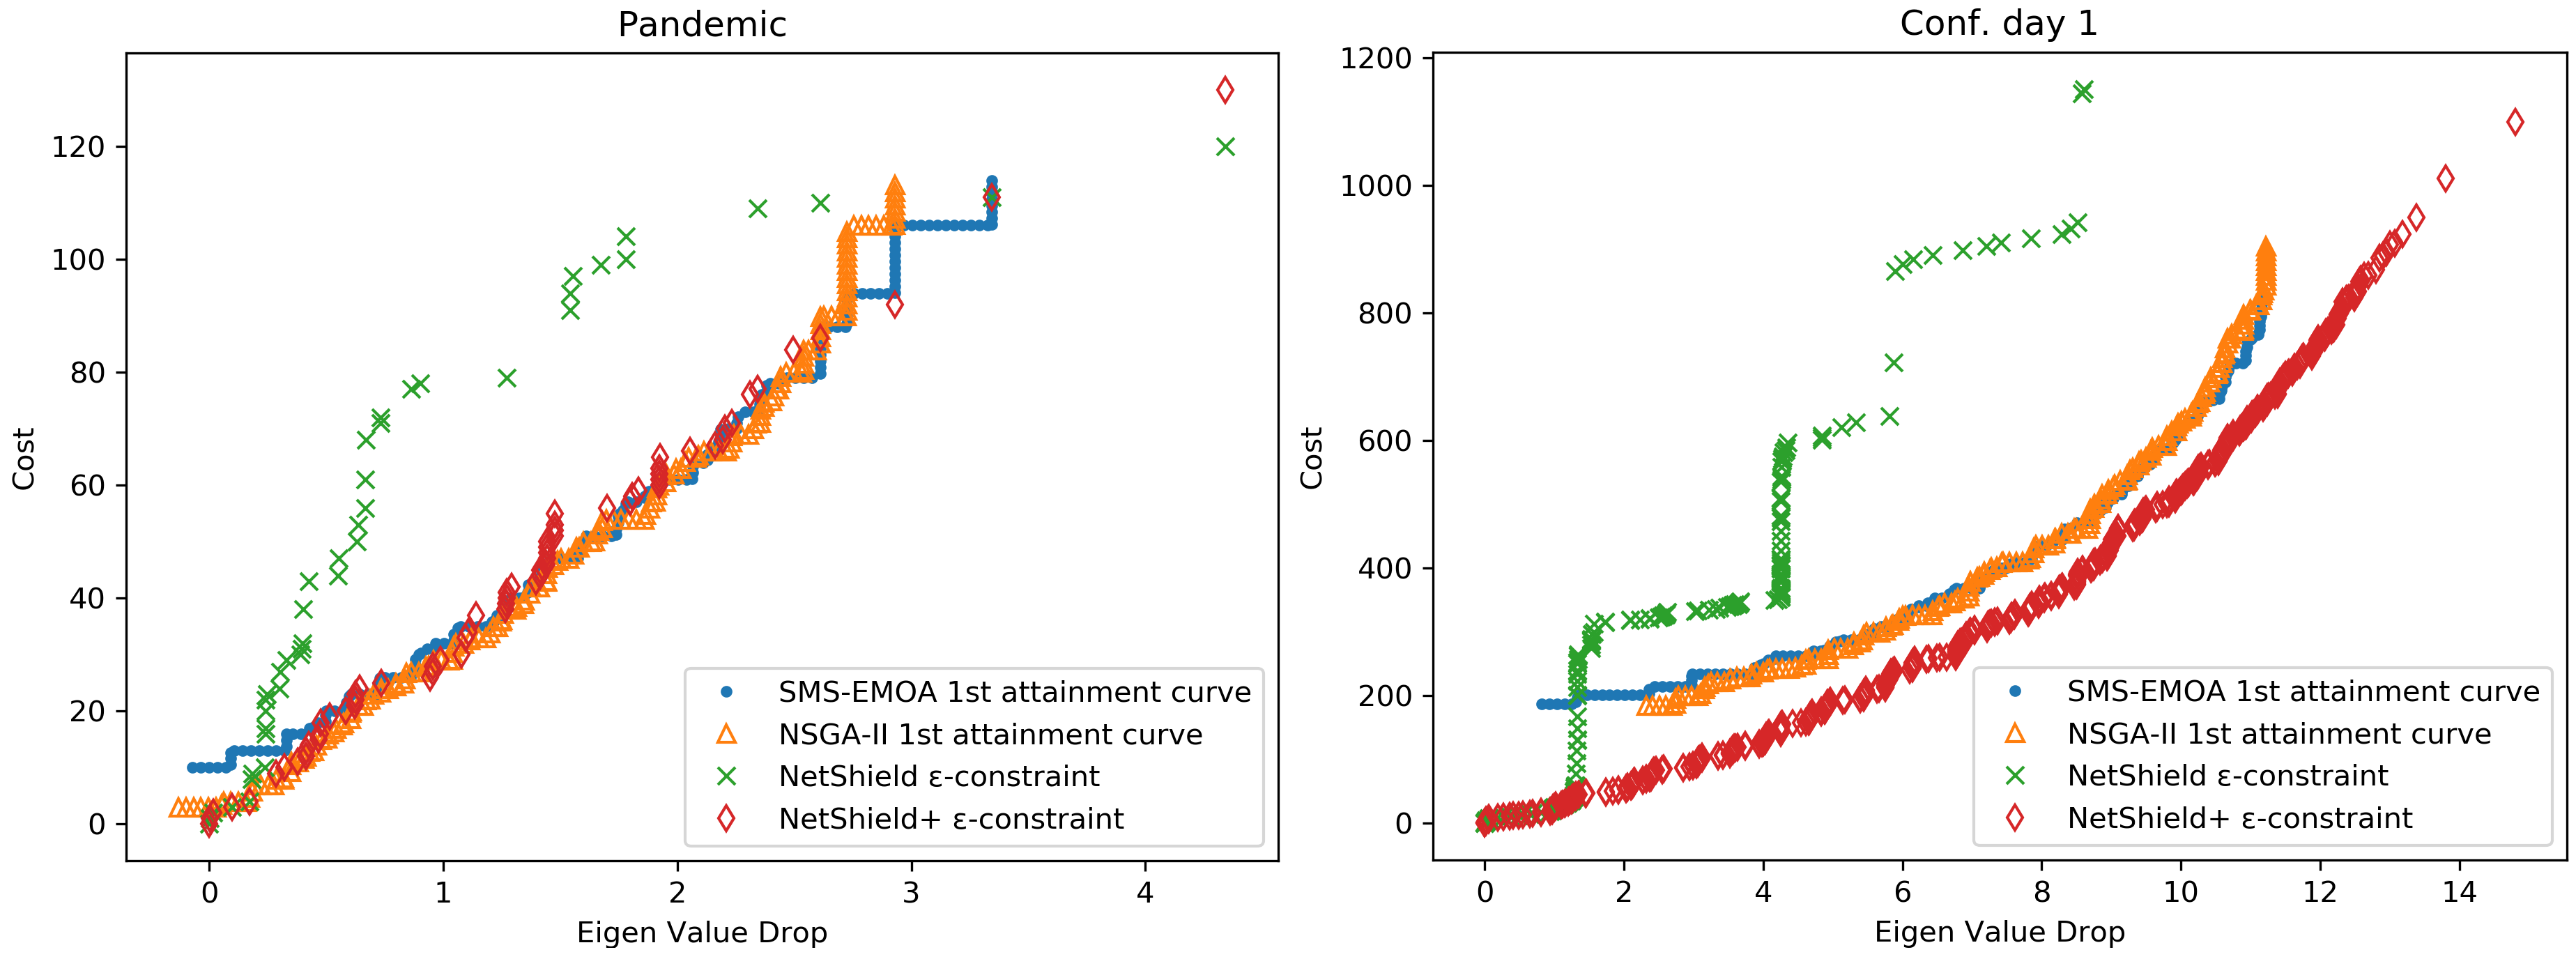
\includegraphics[width=\textwidth]{Images/panconf_attaintment_netshield.png}
  \caption{Results GAs and NetShield(+) with $\epsilon$-constraint method}
  \label{fig:res_panconf}
\end{figure}

\begin{figure}
  \centering
    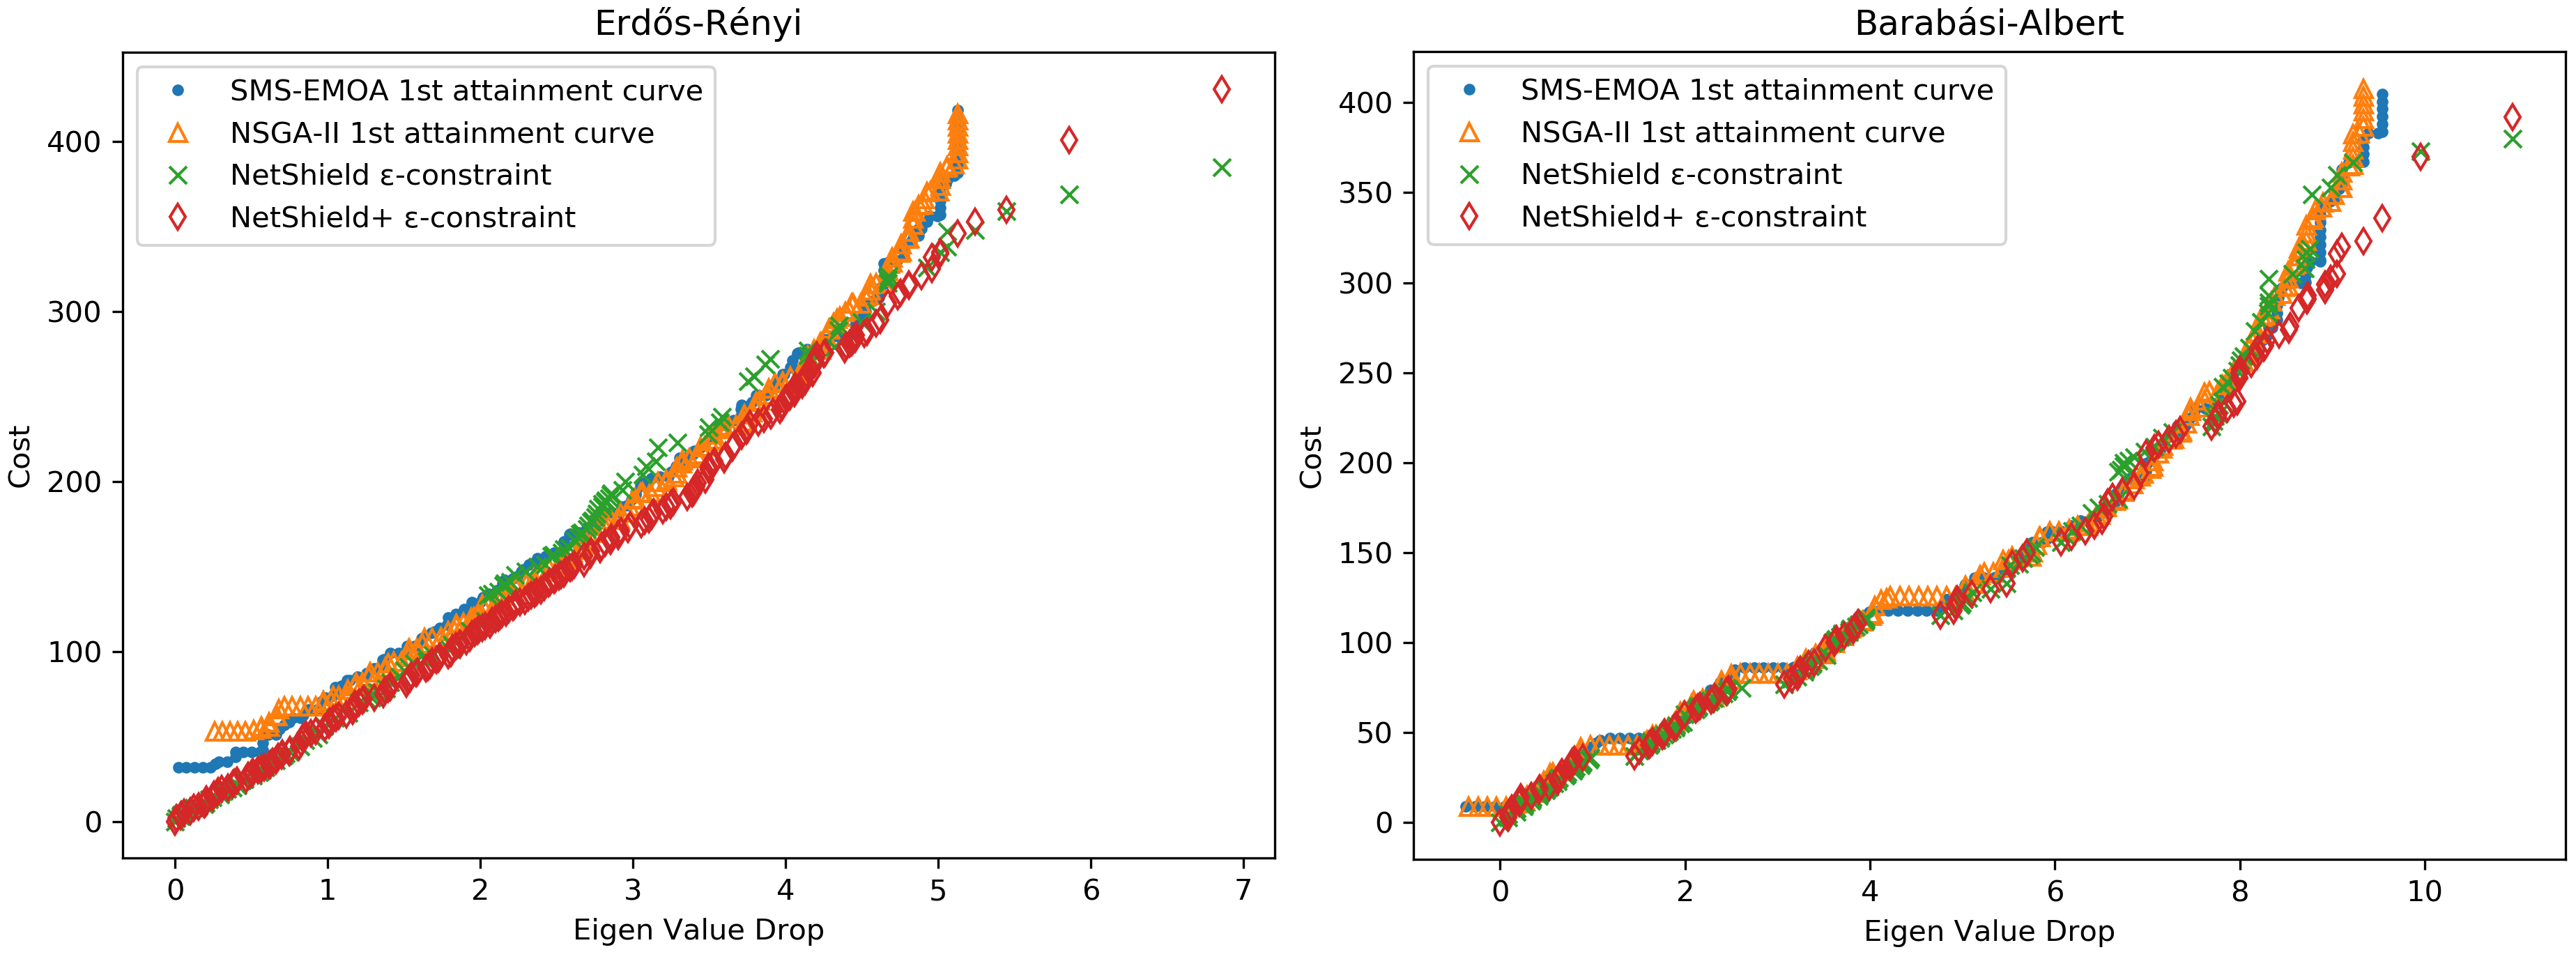
\includegraphics[width=\textwidth]{Images/Erdos_Bara_V100_attaintment_netshield.png}
  \caption{Results GAs and NetShield(+) with $\epsilon$-constraint method}
  \label{fig:res_erbara}
\end{figure}


%\begin{figure}
%\centering
%    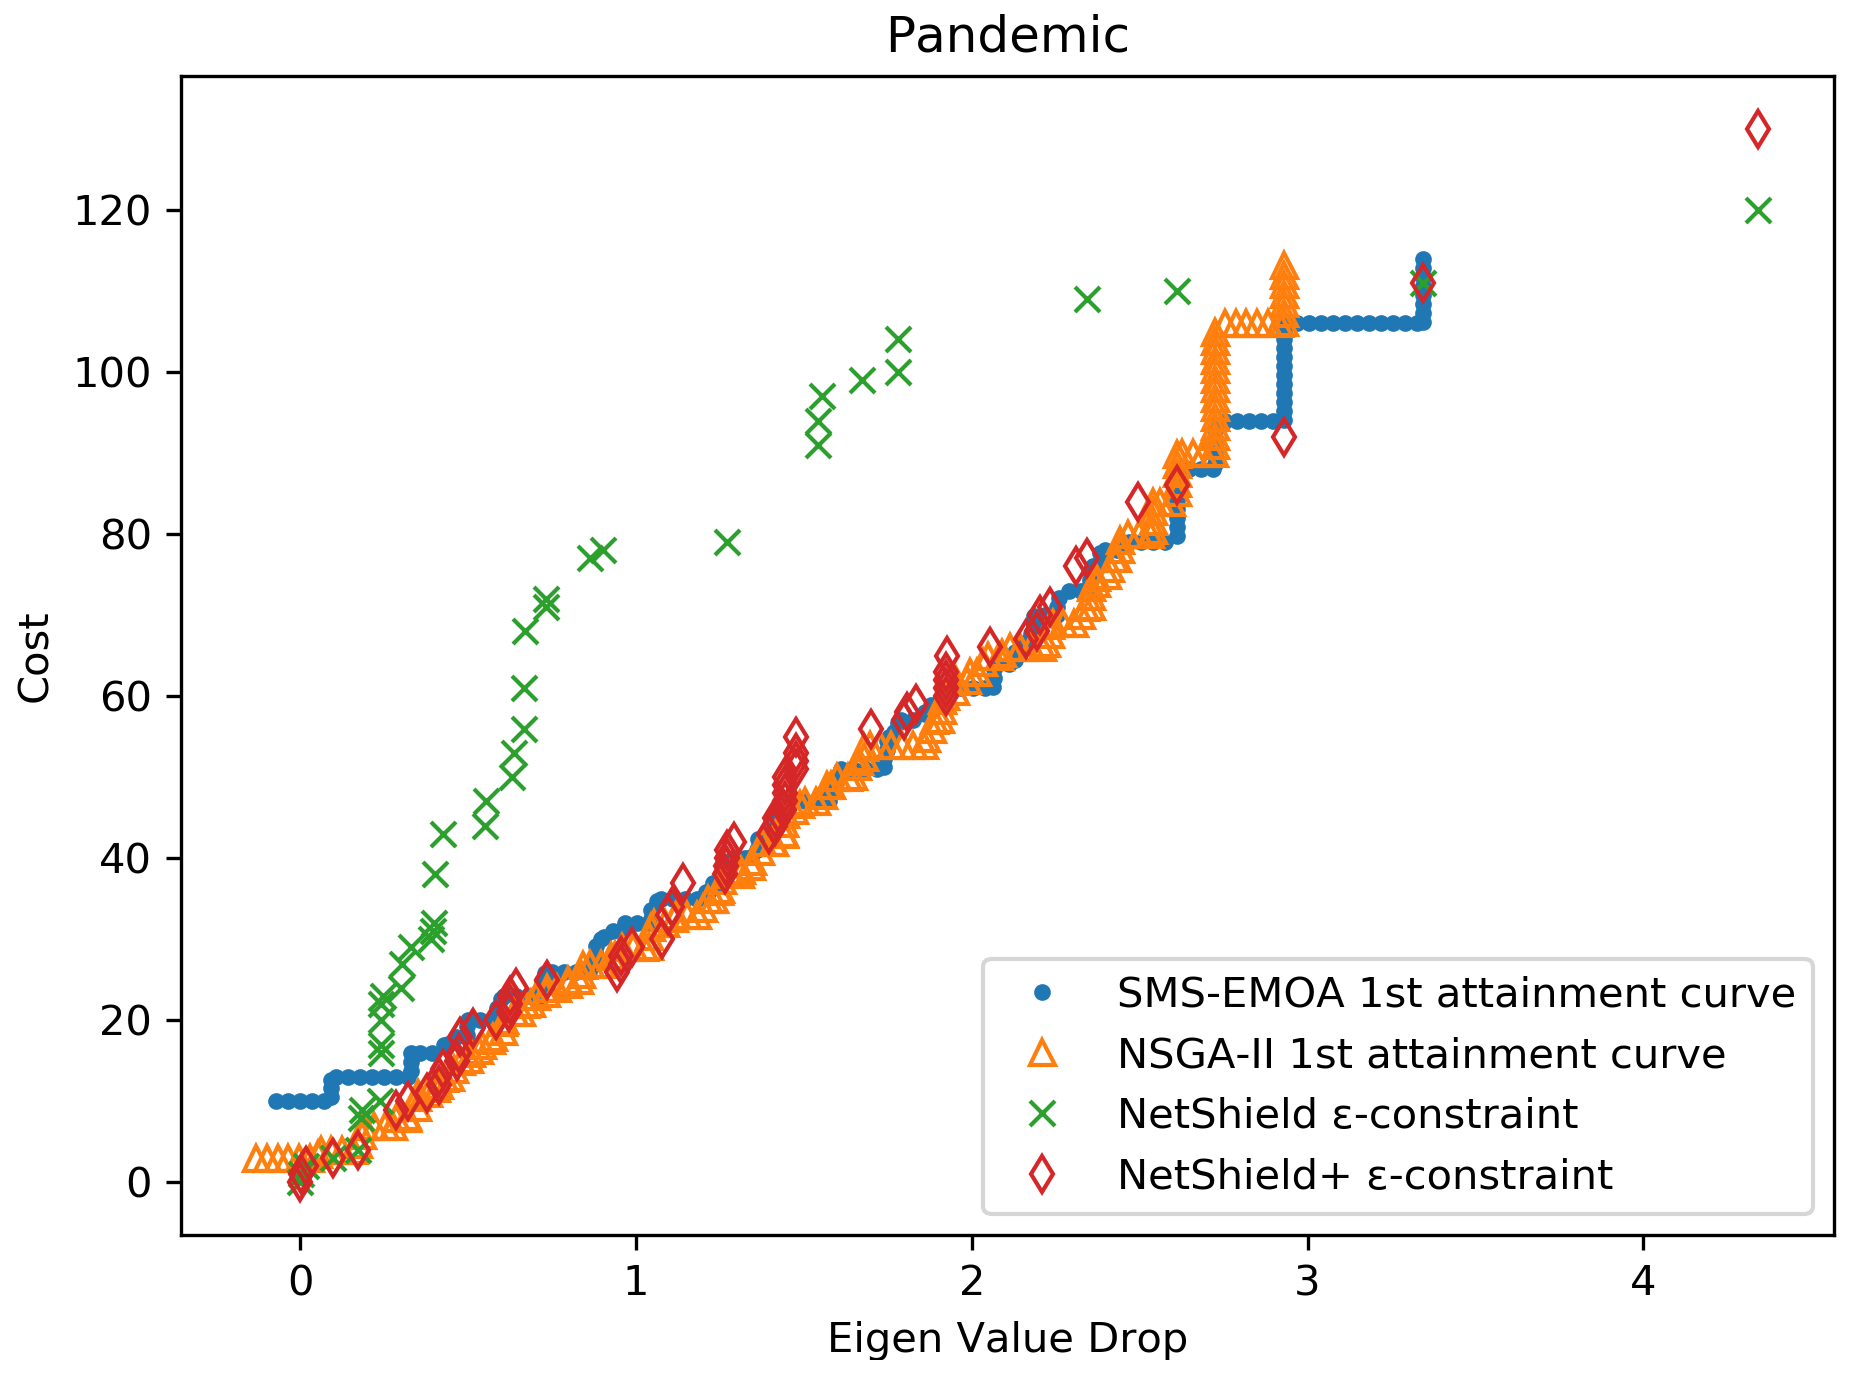
\includegraphics[width=0.95\textwidth]{Images/pandemic_attaintment_netshield.png}
%   \caption{Results GAs and NetShield(+) with $\epsilon$-constraint method}
%  \label{fig:Pandemic_atns}
%\end{figure}

%\begin{figure}
%\centering
%    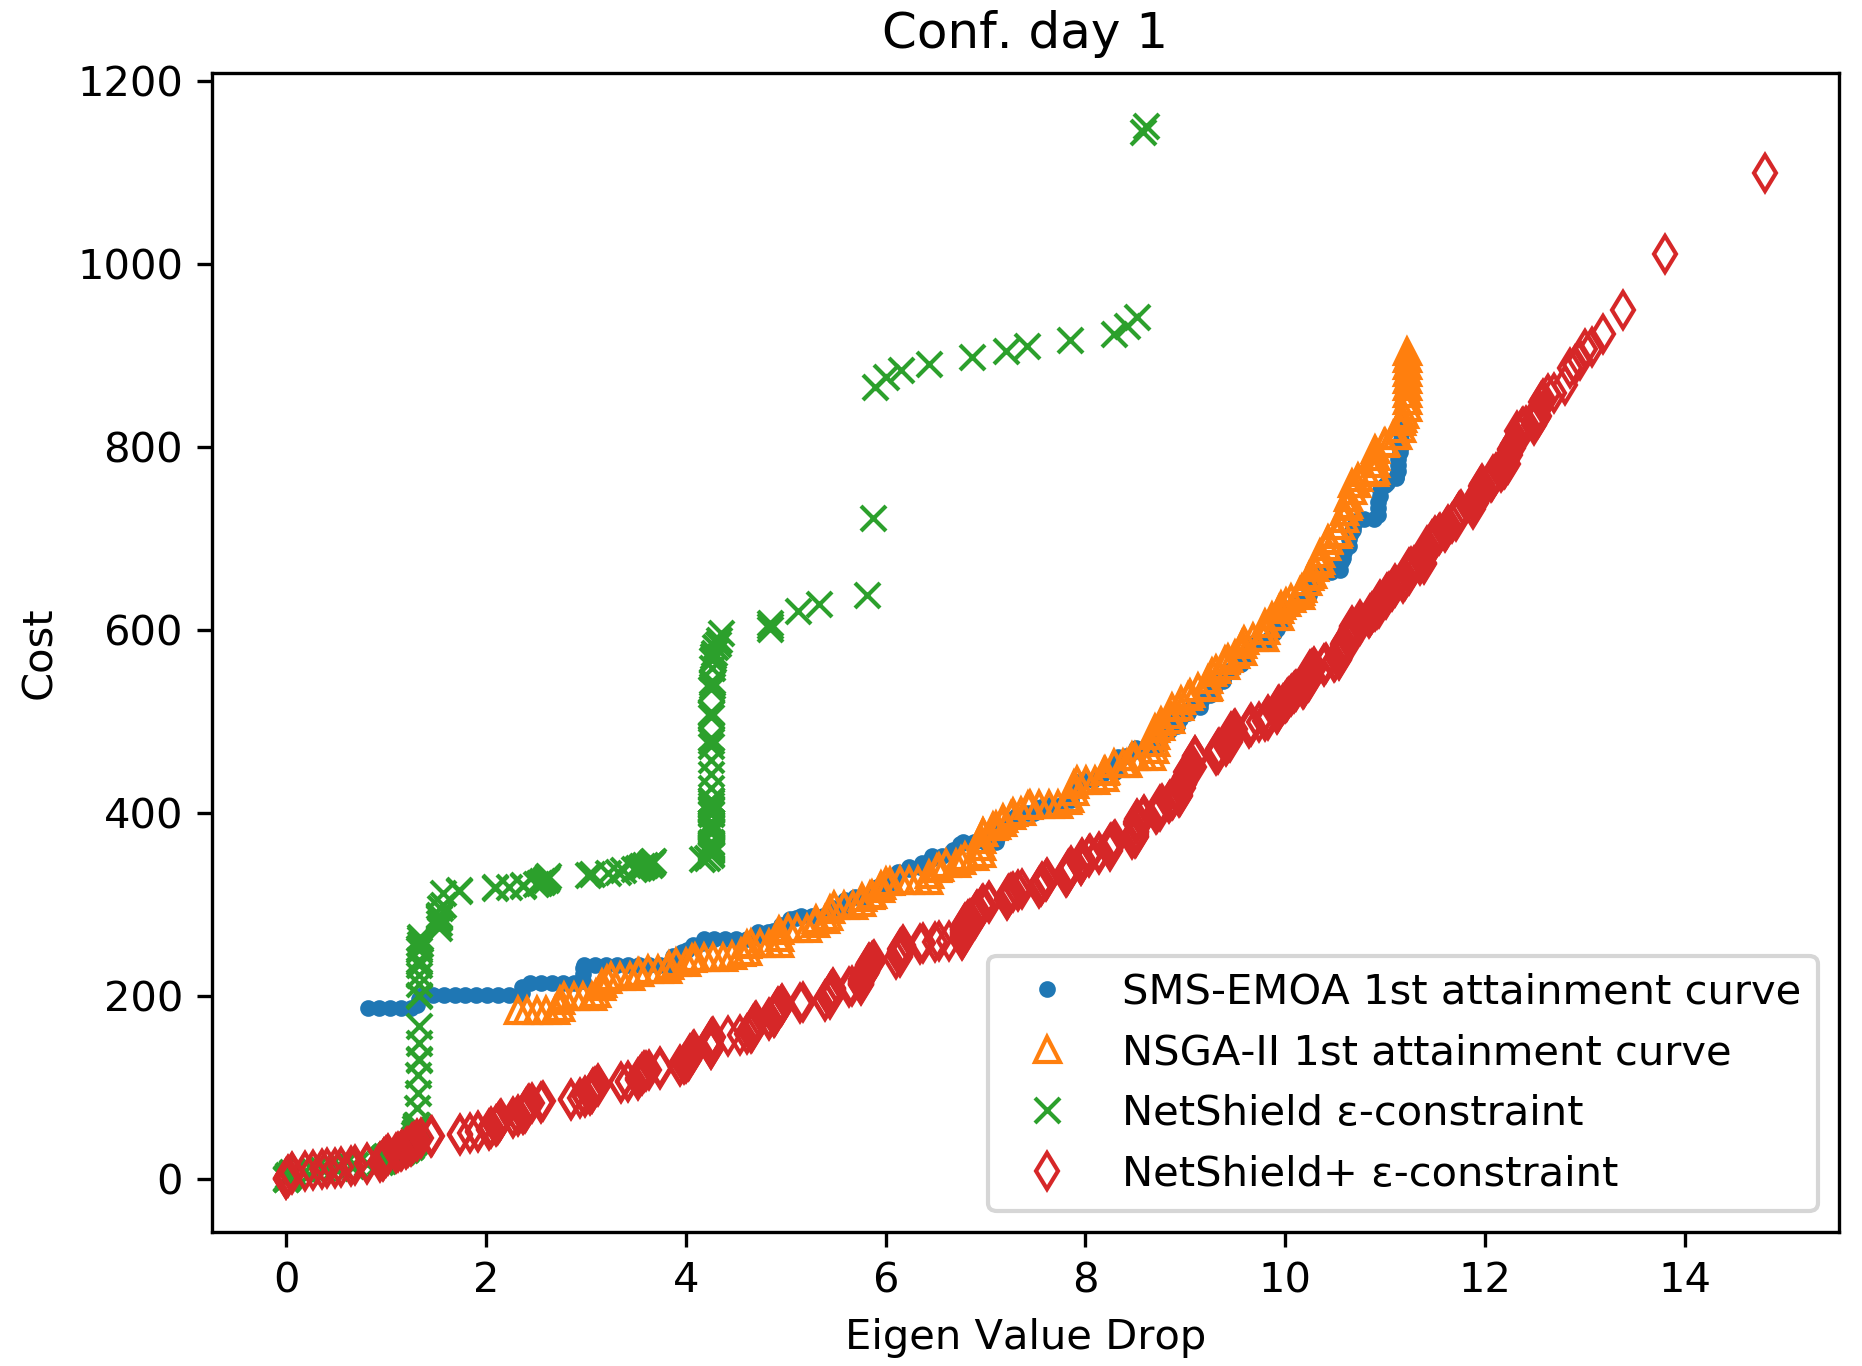
\includegraphics[width=0.95\textwidth]{Images/day1_attaintment_netshield.png}
%    \caption{Results GAs and NetShield(+) with $\epsilon$-constraint method}
%  \label{fig:day1_atns}
%\end{figure}

%\begin{figure}
%  \centering
%    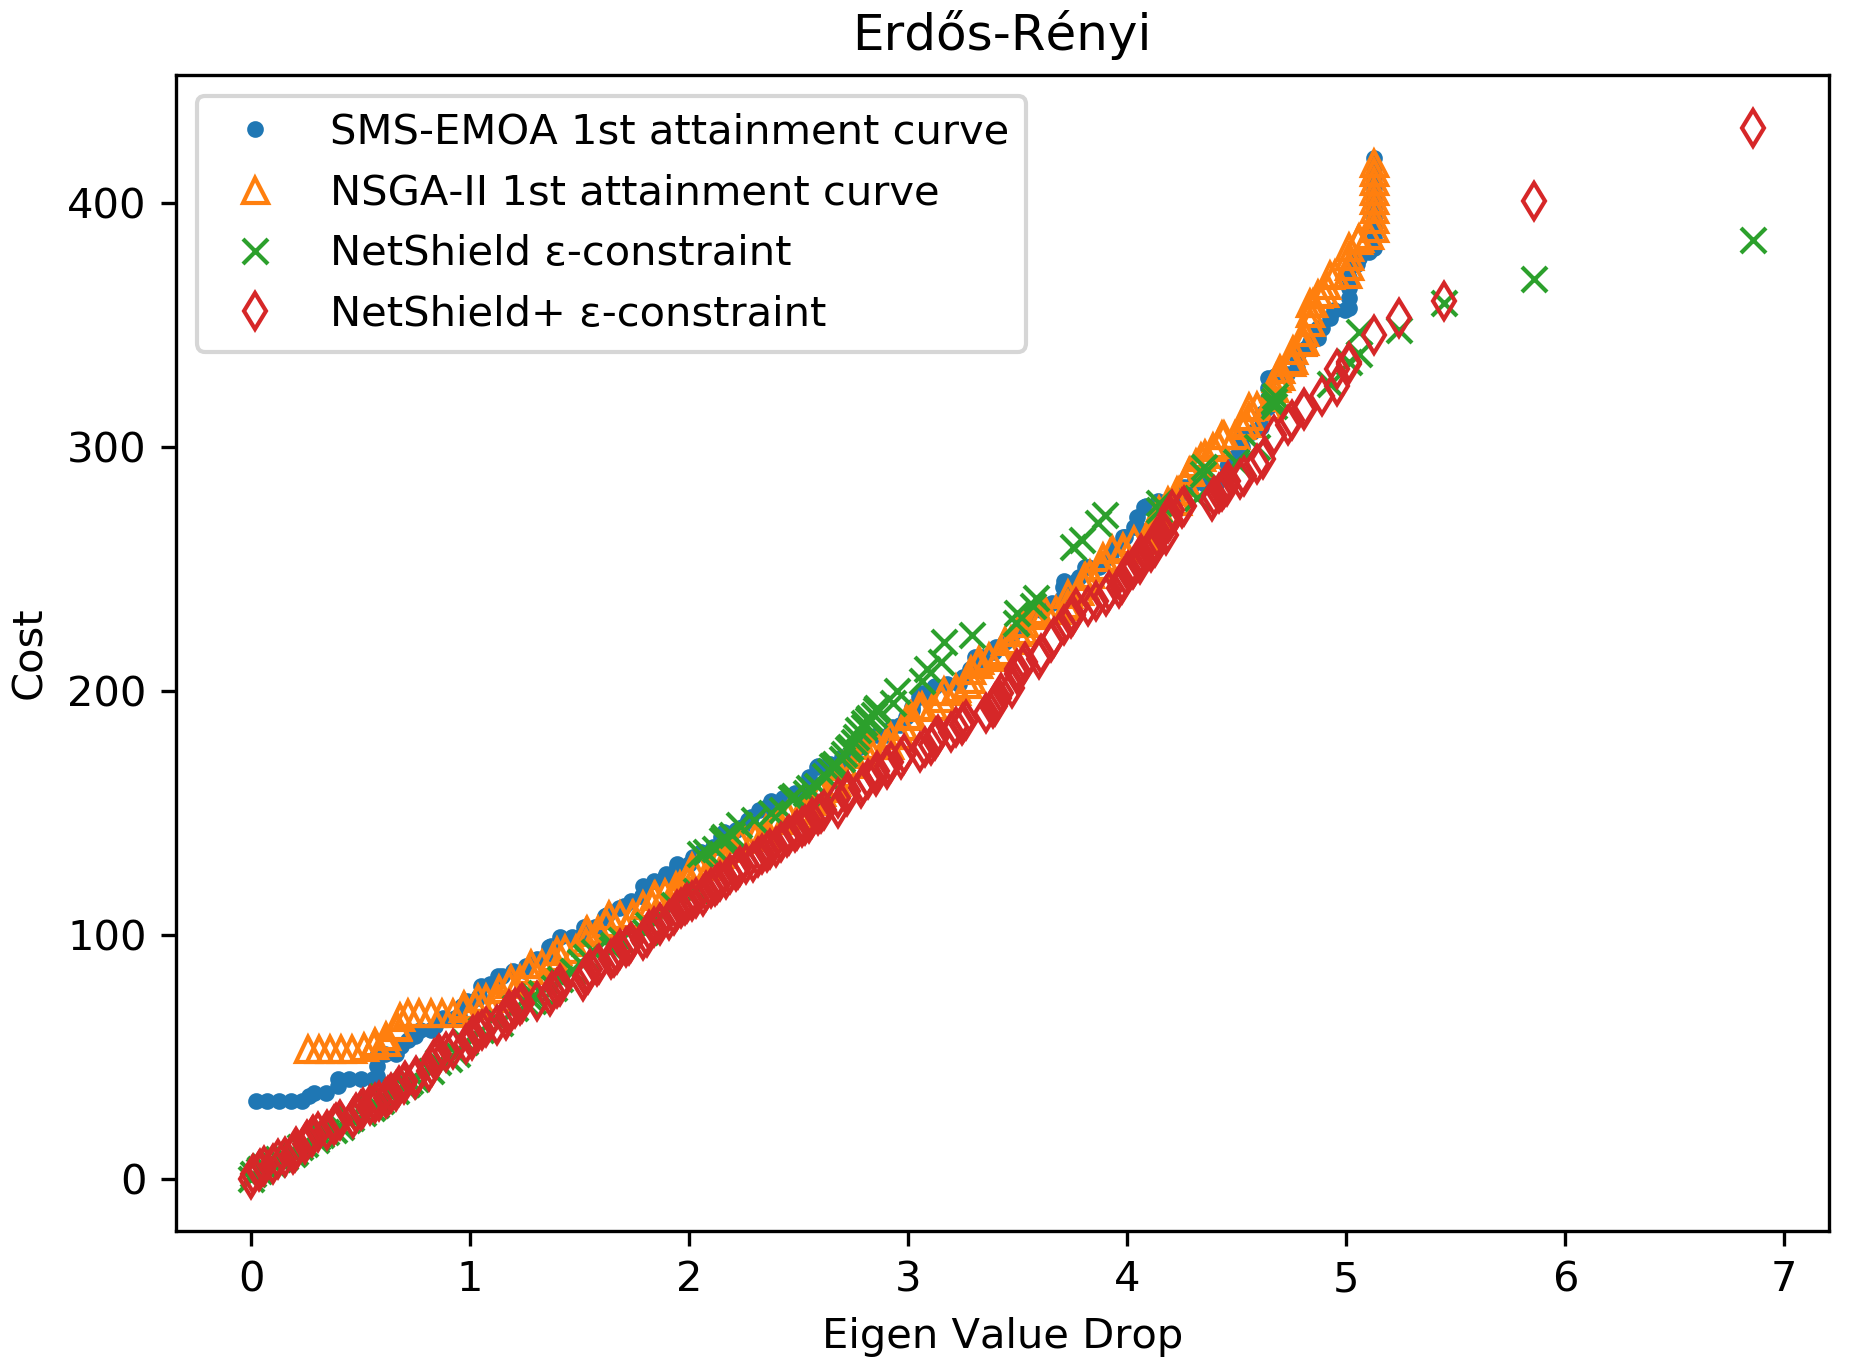
\includegraphics[width=0.95\textwidth]{Images/Erdos_Renyi_V100_attaintment_netshield}
%  \caption{Results GAs and NetShield(+) with $\epsilon$-constraint method}
%  \label{fig:erdos_renyi_atns}
%\end{figure}

%\begin{figure}
%  \centering
%    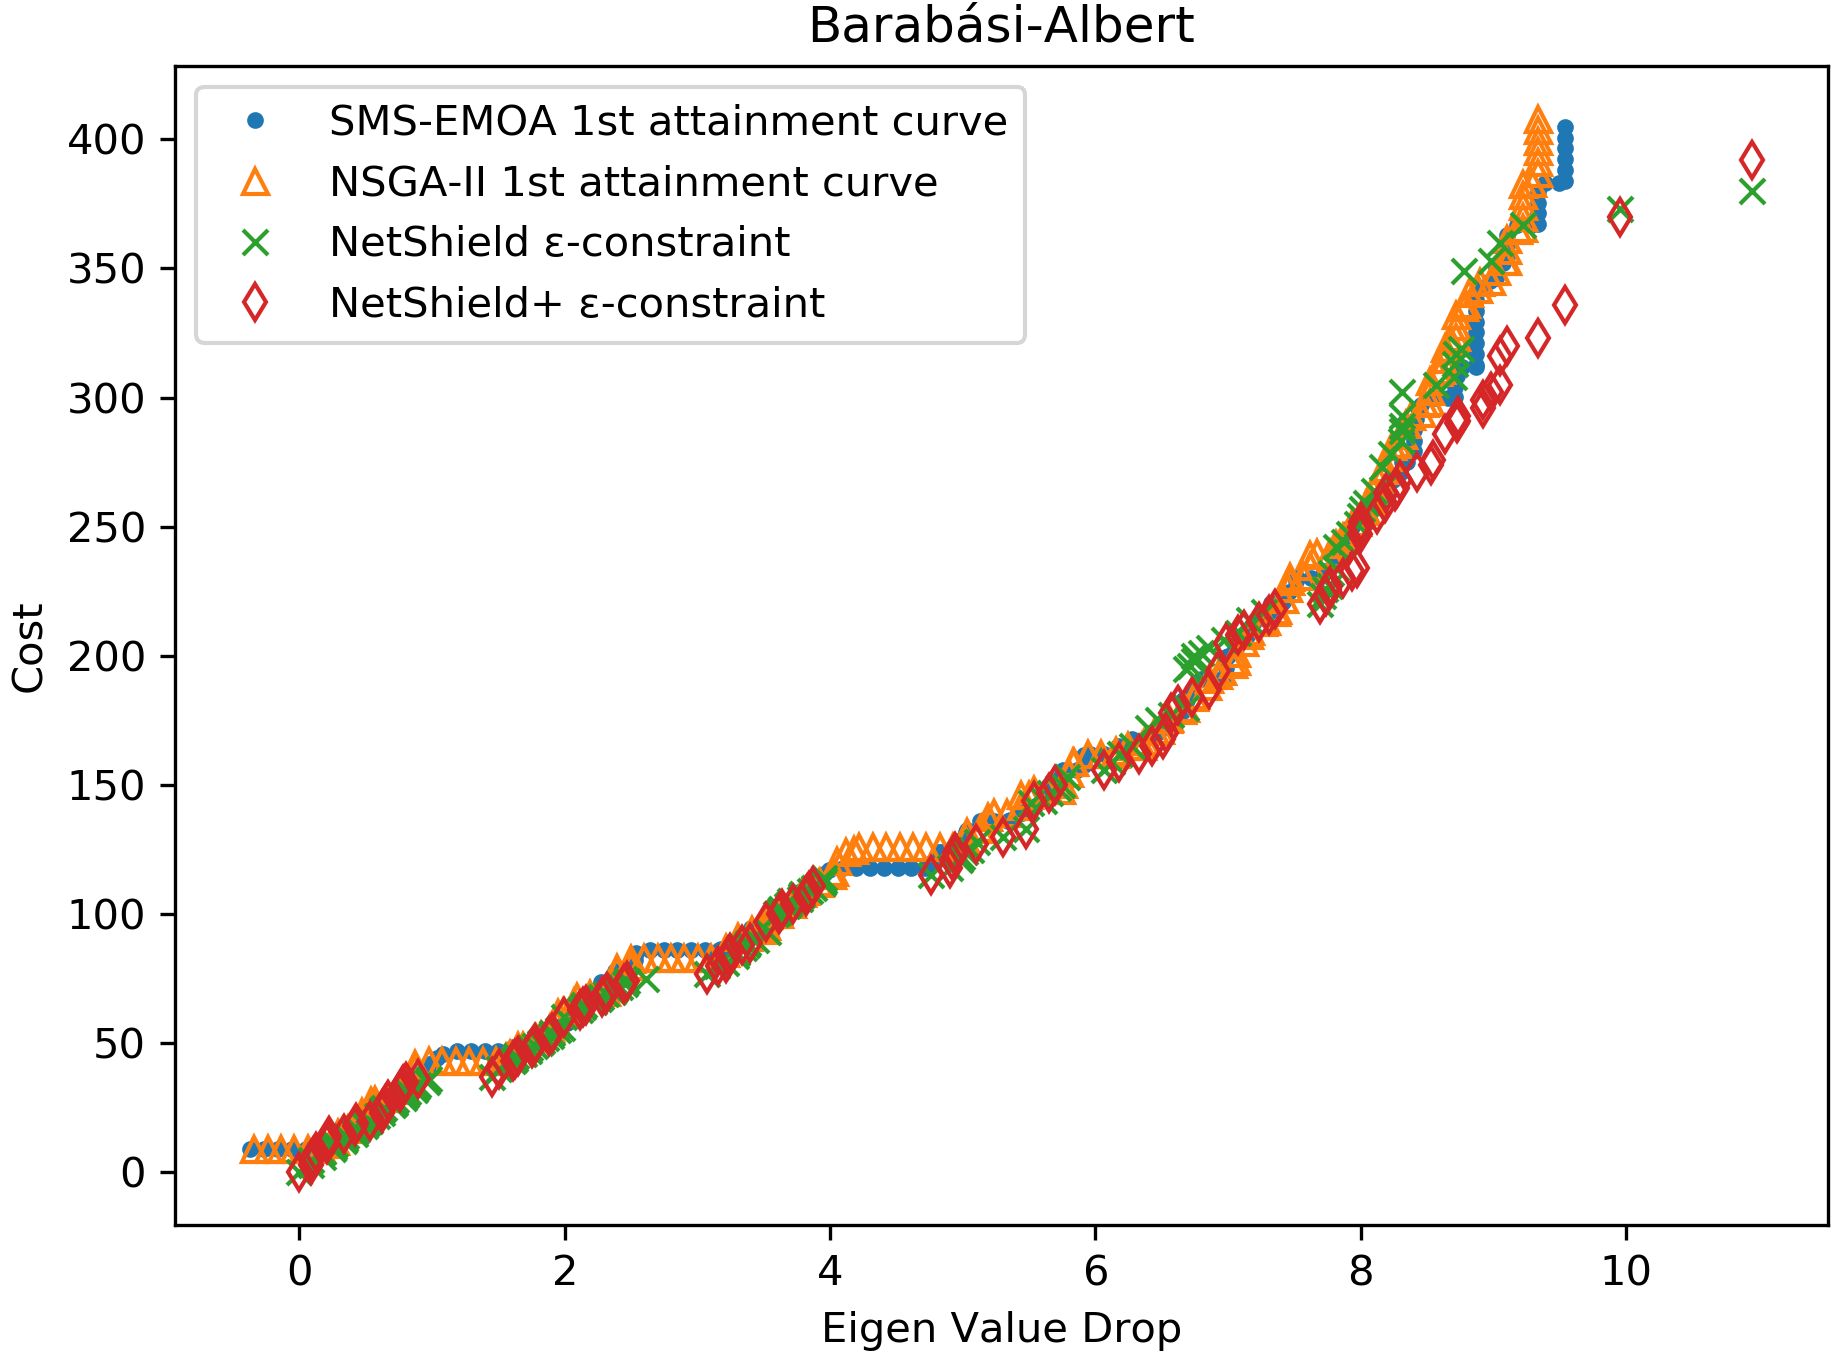
\includegraphics[width=0.95\textwidth]{Images/Barabasi_Albert_V100_attaintment_netshield}
%  \caption{Results GAs and NetShield(+) with $\epsilon$-constraint method}
%  \label{fig:baral_atns}
%\end{figure}

\begin{figure}
  \centering
    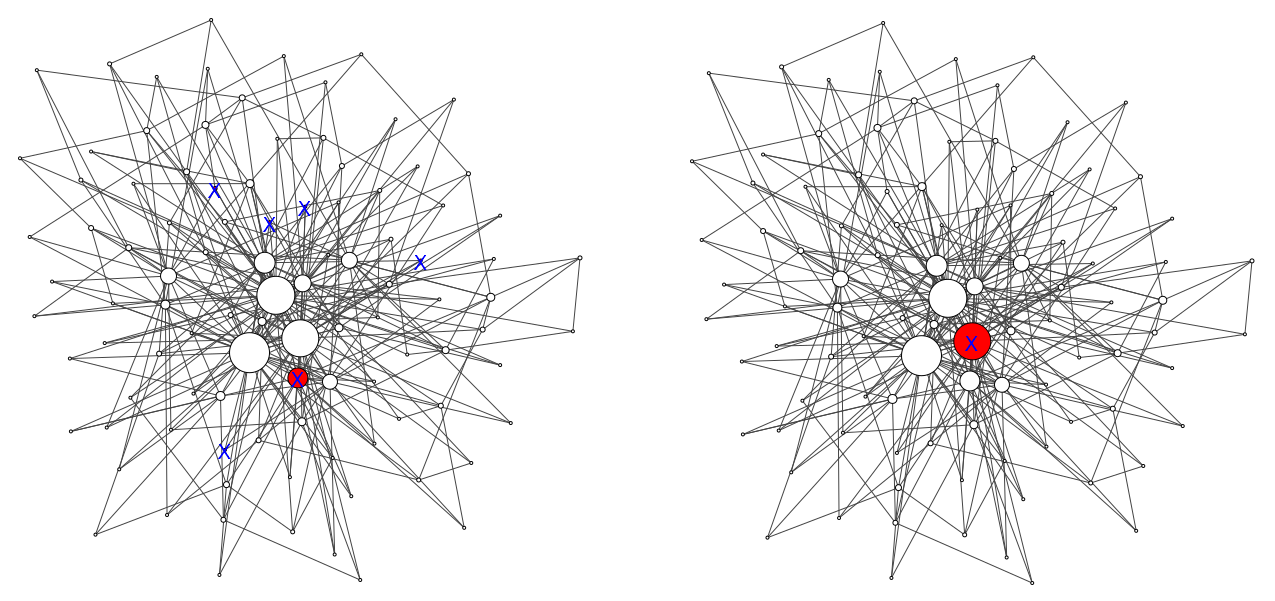
\includegraphics[width=\textwidth]{Images/j1}
    \caption{Selected nodes are red and denoted with $\times$. Nodes have been scaled with degree. Left: 6 selected nodes, cost of 36, $\Delta\lambda$ of 0.975.
            Right: 1 selected node, cost of 37, $\Delta\lambda$ of 1.455}
  \label{fig:bara_j1}
\end{figure}

\FloatBarrier

\subsection{Hybrid GA approach}

The results for the GAs initialised with the results from the NetShield methods for the Pandemic and Barab\'asi-Albert graph are shown in Figure \ref{fig:res_atins}. They are shown together with the initialisation sets. The most notable improvements found by the GAs are for the Pandemic graph. Here the results of the inaccuracies of the Shield-value have been corrected. It appears that in these cases, the GAs have the ability to repair such issues.

The improvements for the Barab\'asi-Albert graph are more minor. Either the initialisation sets are already close to the Pareto fronts or there may not be enough diversity in the initial populations for the GAs to find better solutions.

\begin{figure}
  \centering
    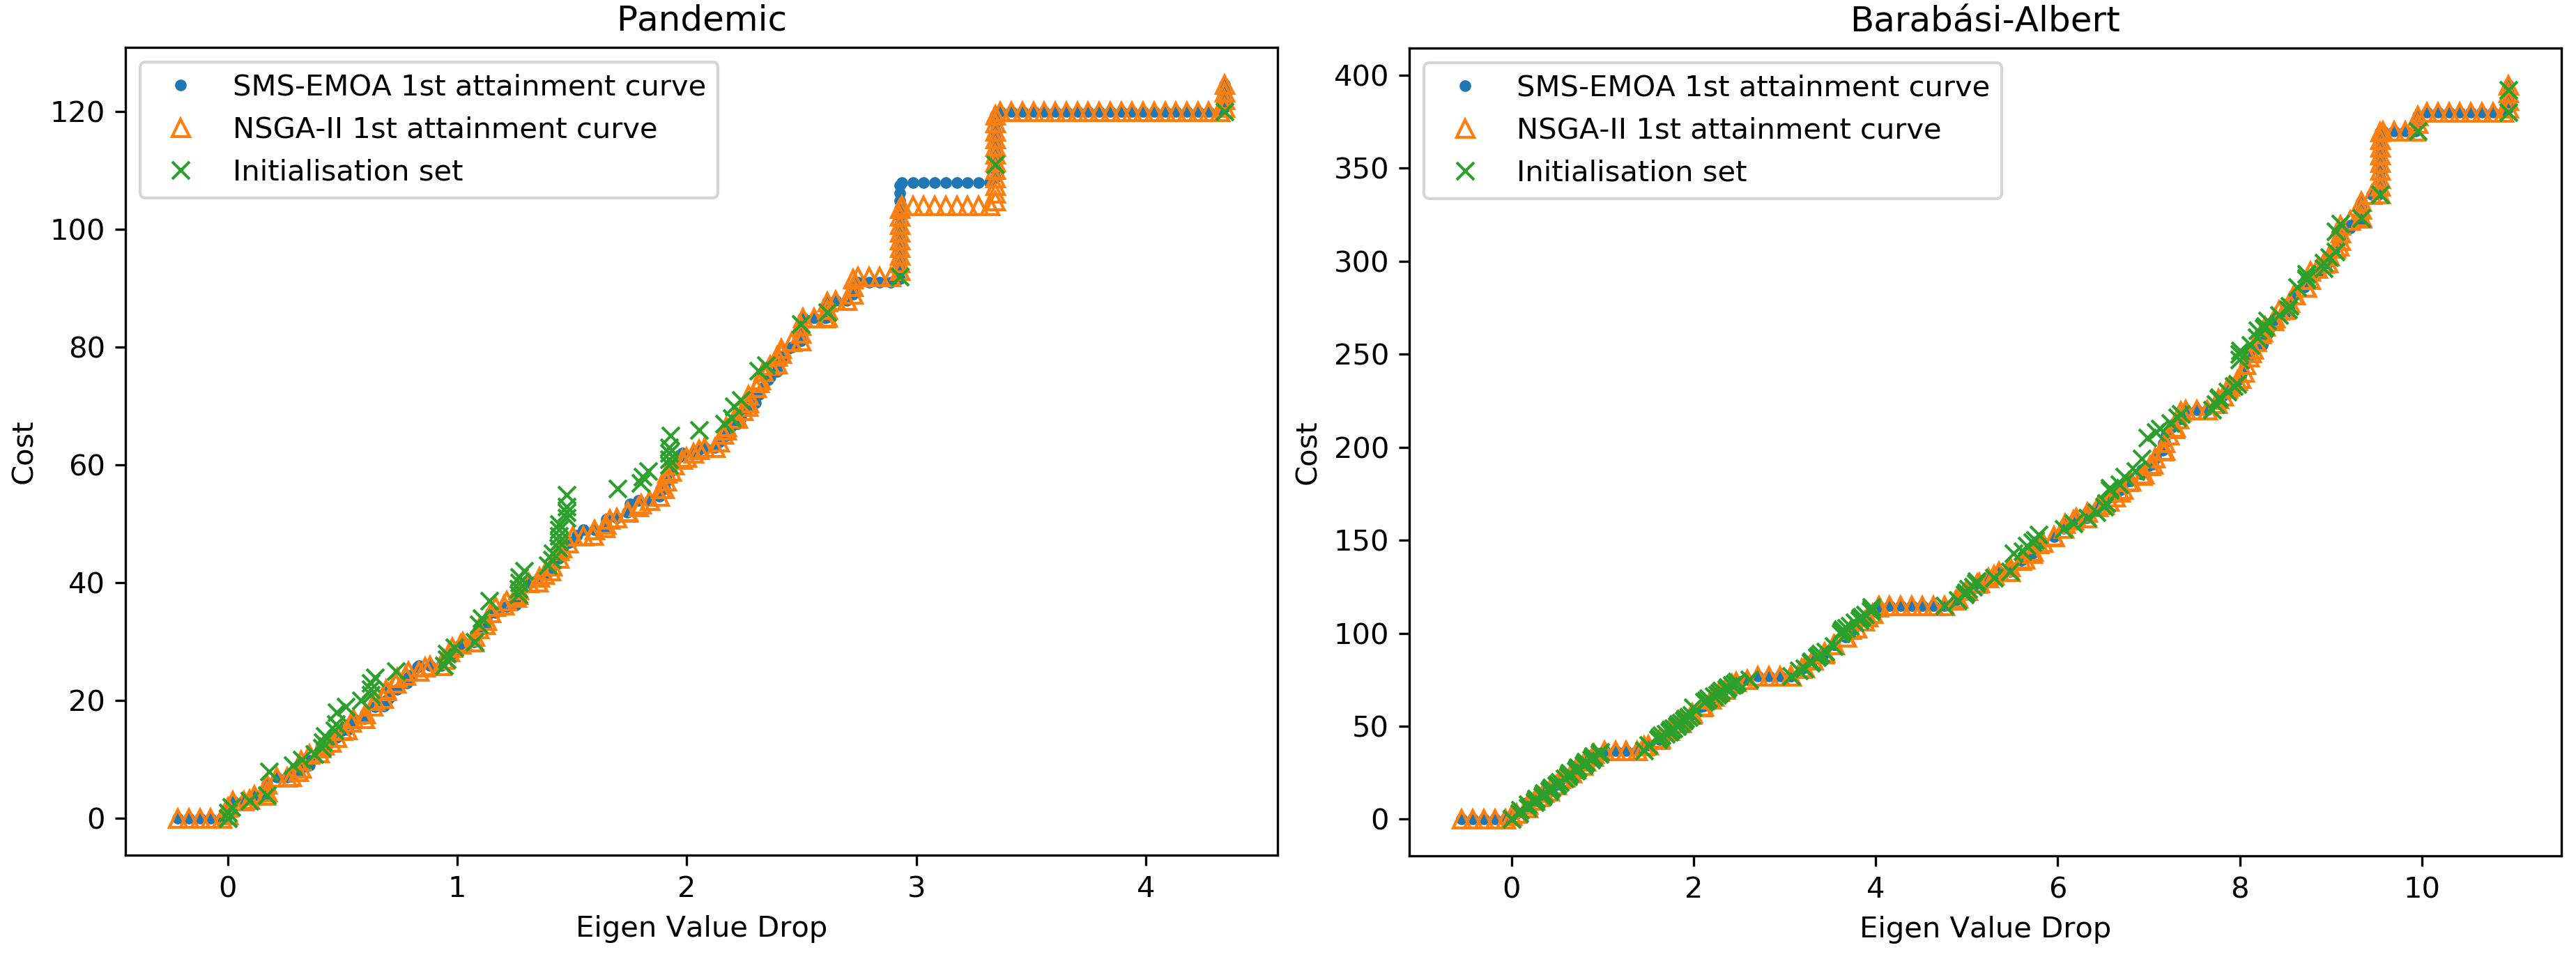
\includegraphics[width=\textwidth]{Images/pandbara_attainment_nsinit}
  \caption{Results hybrid GAs}
  \label{fig:res_atins}
\end{figure}

\section{Conclusion}

In this paper, it is shown that the NetShield and NetShield+ algorithms can be extended with an $\epsilon$-constraint method, using an exact quadratic programming solver (here: Gurobi). In this manner, a multi-objective variant of the node immunisation problem can be solved with a cost function added which is proportional to the effort of the node removal. The performance is mostly equivalent or better than two multi-objective genetic algorithms specifically designed for multi-objective optimisation, except for cases where the Shield-value function is inaccurate due to characteristics of the network. In general the NetShield+ method is more robust than the NetShield method, but there are exceptions. Combining the GAs with the NetShield algorithm as initial population only provided small further improvements. Therefore, if time permits and the most accurate Pareto front approximation is required, a valid approach would be to use all methods and combine the end results.

The results also show that there does not appear to be a typical shape to the Pareto fronts resulting from this problem. They are dependent on both the topology of the network and on the cost function.

It should also be noted, that we focused solely on the eigen-value drop. While this is an effective measure under the SIS infection model, the properties of real world epidemics may not be fully captured solely by this model. Such additional aspects are mentioned, for instance, in \cite{plaat}. In addition, we also assume that any nodes in the network can be immunised. This also may not translate well to real world scenarios. Therefore, future work should also take a broader view of the problem than further improving the eigen-drop via the process of node removal.

\addcontentsline{toc}{section}{References}

\bibliographystyle{abbrv}
\bibliographystyle{unsrt}
\bibliography{bibliography}

\end{document}
